%---------------------------------------------------------------------------------------------------
% Introduction
%---------------------------------------------------------------------------------------------------
\newpage
%\part{start}
\chapter{Introduction}

	The main objective that I had to accomplish for the navigation module was, to connect the google direction API \cite{googleDirecAPI}. 
	This sub-module is responsible for sending queries based upon users current location and the end destination. 
	The queries will be resolved in the state of the art google servers where the 
	routes will be calculated using advanced algorithms and the massive amount of data that google possess. 

	\begin{figure}[htbp!]
		\centering 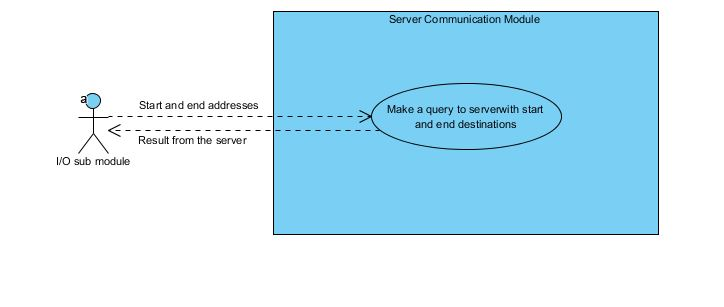
\includegraphics[scale=0.7]{grafiken/googleServerCommunication.jpg}
		\caption{Use case diagram: Google API sub-module communication}
		\label{fig:Google API communication}
	\end{figure}

	\par
	From the figure \ref{fig:Google API communication} it can be a seen that the API sub-module is 
	just an interface which communicates with the server to provide the calculated is a 
	middleware between the server and the navigation. 
	
	\section{Why I choose this package}
	The major focus of my objectives were related to the software engineering aspects instead of
	the hardware side. Personally I opted to go to this direction because I believe that software
	design is an important part of every project and it has always been a challenge to design a project base
	in a way which is robust, scalable and can be maintained with ease. By choosing this package,
	I had the flexibility to develop a system by applying the software design patterns and experiment with 
	the new	technologies available and see them in practice including, what are their pros and cons. 